\documentclass[11pt,a4paper]{book}

\usepackage{pdfsync}		% Texshop feature: reach source by command-clicking PDF
\usepackage{graphicx}
\usepackage{floatflt}			% Figures with text flowing around them
\usepackage{rotating}
\usepackage{amsmath}		% Extra math stuff (align for equations, etc.)
\usepackage{exercise}		% For writing exercises, answers collected in .ans file
\usepackage{verbatim}		% Needed for exercise.sty functionality
%\usepackage{nftimes}
\usepackage{apalike}
\usepackage{fancyhdr}		% Decorative lines and headers/footers
\pagestyle{fancy}
\usepackage{makeidx}		% making an index. run "makeindex" and then use \printindex to place index.
\makeindex				% use \index{word} to add an entry for word.
\usepackage{url}			% Print URLs in a rational way

\usepackage[colorlinks=true,urlcolor=blue,linkcolor=blue]{hyperref}		% Make clickable URLs

% Stuff to do with exercise.sty. Old package, maybe find newer one?
% Answers are put in .ans file which can then be included!!
%\numberexercises{chapter}
%\exercisehead{\bf$\bullet$\,Exercise }{:}


% Trick for getting decorative line to overhang margin (from fancyhdr documentation)
\addtolength{\headwidth}{\marginparsep}
\addtolength{\headwidth}{\marginparwidth}

\newcommand{\ie}{\emph{i.e.},\ }
\newcommand{\eg}{\emph{e.g.},\ }
\newcommand{\etc}{\emph{etc.}}
\newcommand{\e}{\emph}


\begin{document}

\title{\Huge \bf Lecture Notes on Evolutionary Theory and Population Genetics\\{\Large Version 2.0.1} }
\author{\Large \bf Anders Gorm Pedersen\\Technical University of Denmark}
\maketitle

\fancyhead{}
\fancyfoot{}
\fancyhead[LE,RO]{\thepage}		
\renewcommand{\headrulewidth}{0.4pt}
\fancypagestyle{plain}{\fancyhead[LO,RE]{}}

\frontmatter
	\tableofcontents 

\mainmatter

%%%%%%%%%%%%%%%%%%%%%%%%%%%%%%%%%%%%%%%%%%%%%
%							CHAPTER
%%%%%%%%%%%%%%%%%%%%%%%%%%%%%%%%%%%%%%%%%%%%%

\chapter{Brief Introduction to Evolutionary Theory}
		\fancyhead[LO]{Chapter 1: Brief Introduction to Evolutionary Theory}		
		\fancyhead[RE]{Molecular Evolution, lecture notes}
		\fancyfoot[LO,RE]{\footnotesize  \  Anders Gorm Pedersen, \the\year{}}
		%\clearpage
		
\section{Classification}

One of the main goals of early biological research was classification\index{Classification}, \ie the systematic arrangement of living organisms into categories reflecting their natural relationships. The most successful system was invented by the swede Carl Linnaeus\index{Linnaeus}\index{Linn\'e}, and presented in his book 
"Systema Naturae" first published in 1735. The system we use today is essentially the one devised by Linnaeus. It is a hierarchical system with seven major ranks: kingdom\index{Kingdom}, phylum\index{Phylum}, class\index{Class}, order\index{Order}, family\index{Family}, genus\index{Genus}, and species\index{Species}. 

\marginpar{
\resizebox{0.8\marginparwidth}{!}{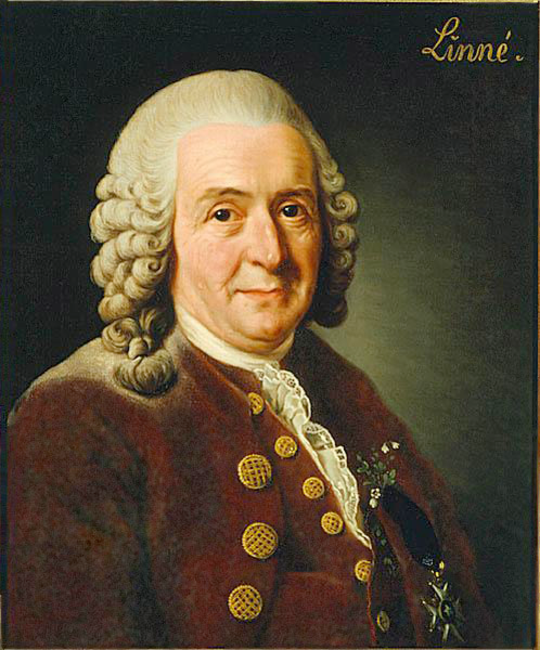
\includegraphics{figs/linnaeus.pdf}}\\
\small Carl~Linnaeus\\ (1707--1778)\\ 
(\small \href{http://commons.wikimedia.org/wiki/File:Carolus_Linnaeus_(cleaned_up_version).jpg}{Image source})
}


Specifically, groups of similar species are placed together in a genus, groups of related genera are
placed together in a family, families are grouped into orders, orders into classes, classes into phyla, and phyla into kingdoms. When depicted graphically, the Linnean system can be shown in the form of a tree with individual species at the tips, and with internal nodes in the tree representing higher-level categories (Fig. \ref{taxtree}). Along with this classification system, Linnaeus also developed the so-called binomial system\index{Binomial system} \marginpar{\small The Linnean system: \begin{itemize}
\item Kingdom
\item Phylum
\item Class
\item Order
\item Family
\item Genus
\item Species
\end{itemize}
}
in which all organisms are identified by a two-part Latinized name. The first name is capitalized and identifies the genus, while the second identifies the species within that genus. For example the genus \emph{Canis} includes \emph{Canis lupus}, the wolf, and \emph{Canis latrans}, the coyote. (\emph{Canis lupus familiaris}, the domestic dog, is now known to be a sub-species of the wolf). Similarly, the genus \emph{Vulpes} contains \emph{Vulpes vulpes}, the red fox, \emph{Vulpes chama} the Cape fox, and others. Both genera (\e{Canis} and \e{Vulpes}) belong to the family \emph{Canidae}, which in its turn is part of the order \emph{Carnivora}, the carnivores. 

Note that it is non-trivial to come up with a generally applicable definition of what exactly a ``species'' is. According to the so-called biological species concept, a species is a group of ``actually or potentially interbreeding natural populations which are reproductively isolated from other such groups''. This definition is due to the evolutionary biologist Ernst Mayr (1904--2005) and is perhaps what most people intuitively understand by the word ``species''. However, the biological species concept does not address the issue of how to define species within groups of organisms that do not reproduce sexually (\eg bacteria), or when organisms are known only from fossils. An alternative definition is the morphological species concept which states that ``species are groups of organisms that share certain morphological or biochemical traits''. This definition is more broadly applicable, but is also far more subjective than~Mayr's.
\begin{figure}[!t]
\begin{center}
\resizebox{\textwidth}{!}{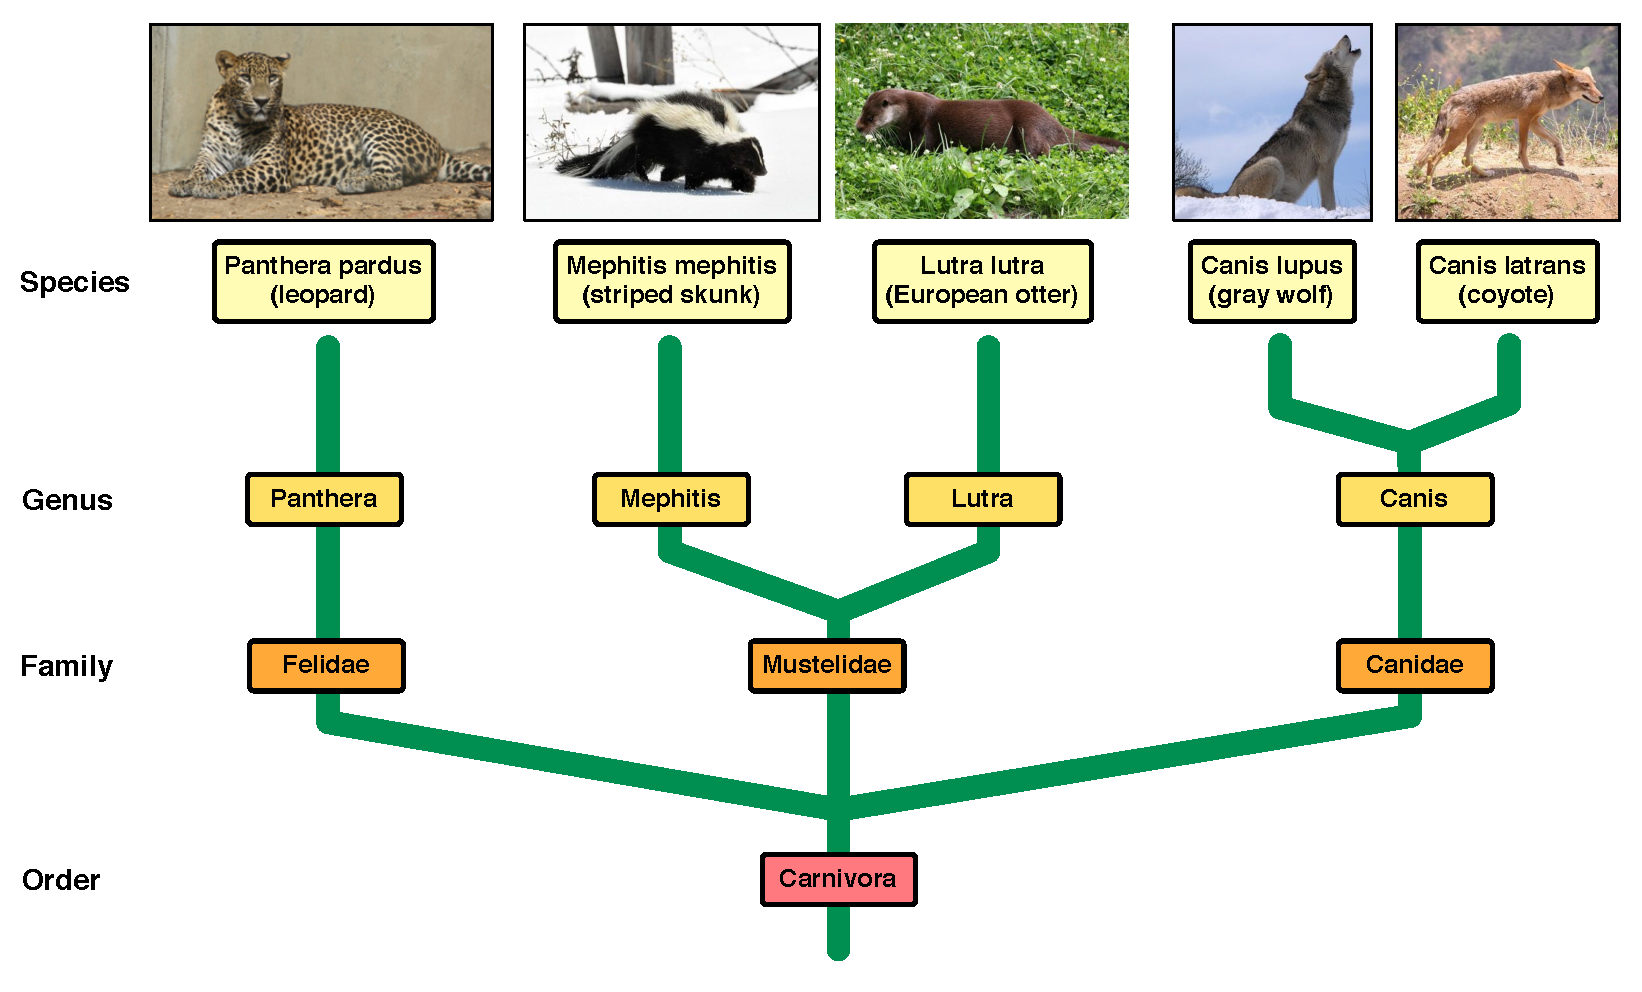
\includegraphics{figs/classification_tree.pdf}}
\caption{\small Linnean classification depicted in the form of a tree.
(Image sources:
 \href{http://commons.wikimedia.org/wiki/File:SriLankaLeopard-ZOO-Jihlava.jpg}{1},
 \href{http://commons.wikimedia.org/wiki/File:Striped_Skunk_(Mephitis_mephitis)_DSC_0030.jpg}{2},
 \href{http://commons.wikimedia.org/wiki/File:Lutra_lutra_2_-_Otter,_Owl,_and_Wildlife_Park.jpg}{3},
 \href{http://en.wikipedia.org/wiki/File:Howlsnow.jpg}{4},
 \href{http://commons.wikimedia.org/wiki/File:Canis_latrans.jpg}{5})
}
\label{taxtree}
\end{center}
\end{figure}

\section{Darwin and the Theory of Evolution}

As mentioned, the Linnean system was highly successful. So much so in fact, that in his publications, Linnaeus provided a survey of all the world's plants and animals as then known---about 7,700 species of plants and 4,400 species of animals..

The first widely accepted scientific explanation for this was given with the 1859 publication of Charles Darwin's\index{Darwin} ``On the Origin of Species'' .  According to Darwin (and others), the ordering principle behind the Linnean system was a history of ``common descent with modification'': all life was believed to have evolved from one---or a few---common ancestors, and taxonomic groupings were simply manifestations of the tree-shaped evolutionary history connecting all present-day species (Fig. \ref{haeckel}). 

The theory of common descent did not in itself address the issue of \emph{how} evolutionary change takes place, but it was able to explain a great deal of puzzling observations.  For instance, similar species are often found in adjacent or overlapping geographical regions, and fossils often resemble (but are different from) present-day species living in the same location. These phenomena are easily explained as the result of divergence from a common ancestor. 
\begin{figure}[!t]
\begin{center}
\resizebox{0.8\textwidth}{!}{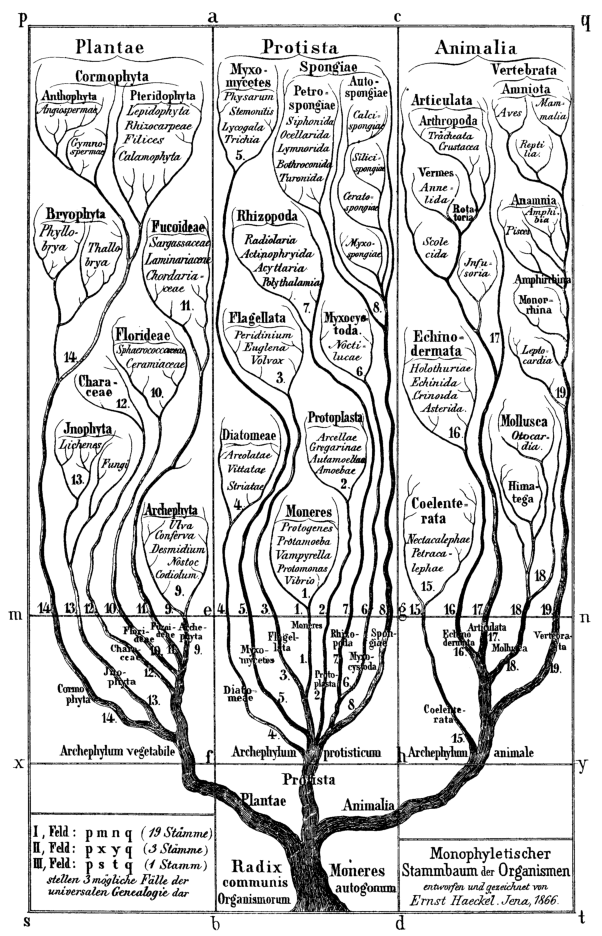
\includegraphics{figs/haeckel.pdf}}
\caption{The tree of life, Ernst Haeckel, 1866
(\href{http://commons.wikimedia.org/wiki/File:Haeckel_arbol_bn.png}{Image source})
}
\label{haeckel}
\end{center}
\end{figure}



\section{Natural Selection}

The mechanism that Darwin proposed for evolutionary change is called {\bf natural selection}\index{Natural selection}. This is related to \index{Artificial selection}artificial selection---the process of intentional (or unintentional) modification of a species through human actions which encourage the breeding of certain traits over others. Examples include crop plants, such as rice and wheat, which have been artificially selected for protein-rich seeds, and dairy cows which have been artificially selected for high milk yields. The wide variety of dog breeds is also a result of artificial selection (for hunting, herding, protection, companionship, and looks) and illustrates that rather significant changes can be obtained in a limited amount of time (many dog breeds were created in the last few hundred years.) You should note that for artificial selection to be possible in the first place, there needs to be naturally occurring and heritable variation in traits of interest: it is only possible to breed high-protein grass sorts, if there are some grass plants that produce more seed protein than others, \emph{and} if that trait is inherited by their descendants.
\marginpar{
\begin{center}
\resizebox{0.7\marginparwidth}{!}{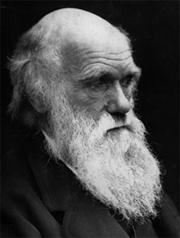
\includegraphics{figs/darwin.jpg}}
\small Charles Darwin\\ (1809-1882)\\
(\small \href{http://commons.wikimedia.org/wiki/File:Charles_Darwin_01.jpg}{Image source})
\end{center}
}


Darwin suggested that a similar process occurs naturally: individuals in the wild who possess characteristics that enhance their prospects for having offspring would undergo a similar process of change over time. Specifically, Darwin postulated that there are four properties of populations that together result in natural selection. These are:
%\begin{quote}
\begin{enumerate}
\item Each generation more offspring is born than the environment can support - a fraction of offspring therefore dies before reaching reproductive age. 
\item Individuals in a population vary in their characteristics.
\item Some of this variation is based on heritable (\emph{i.e.}, genetic) differences.
\item Individuals with favorable characteristics have higher rates of survival and reproduction compared to individuals with less favorable characteristics.
\end{enumerate}
%\end{quote}
If all four postulates are true (and this is generally the case) then advantageous traits will automatically tend to spread in the population, which thereby changes gradually through time. This is natural selection. Let us consider, for instance, a population of butterflies that are preyed upon by birds. Now imagine that at some point a butterfly is born with a mutation that makes the butterfly more difficult to detect (perhaps the coloration of the butterfly's wings becomes darker, thereby better matching the color of the tree trunks on which the butterflies sometimes rest). This butterfly will obviously have a smaller risk of being eaten, and will consequently have an increased chance of surviving to produce offspring. A fraction of the fortunate butterfly's offspring will inherit the advantageous mutation, and in the next generation there will therefore be \emph{several} butterflies with an improved chance of surviving to produce offspring. After a number of generations it is possible that all butterflies will have the mutation, which is then said to be ``fixed''. 

If two sub-populations of a species are somehow separated (for instance due to a geographical barrier), then it is hypothesized that this process may lead to the gradual build-up of differences to the point where the populations are in fact separate species. This process is called speciation\index{Speciation}. (It should be noted that we now know that other evolutionary processes besides natural selection can contribute to speciation).

\section{The Modern Synthesis}

One problem with the theory described in ``Origin of Species'', was that its genetic basis---the nature of heritability---was entirely unknown. In later editions of the book, Darwin proposed a model of inheritance where ``hereditary substances'' from the two parents merge physically in the offspring, so that the hereditary substance in the offspring will be intermediate in form (much like blending red and white paint results in pink paint). Such ``blending inheritance''\index{Blending inheritance} is in fact incompatible with evolution by natural selection, since the constant blending will quickly result in a completely homogeneous population from which the original, advantageous trait cannot be recovered (in the same way it is impossible to extract red paint from pink paint). Moreover, due to the much higher frequency of the original trait, the resulting homogeneous mixture will be very close to the original trait, and very  far from the advantageous one. (In the paint analogy, if one single red butterfly is born at some point, then it will have to mate with a white butterfly resulting in pink offspring. The offspring will most probably mate with white butterflies and their offspring will be a \e{lighter} shade of pink, \etc, \etc \ In the long run, the population will end up being a very, very light shade of pink, instead of all red). 


However, as shown by the Austrian monk Gregor Mendel\index{Mendel}, inheritance is in fact particulate in nature: parental genes do not merge physically; instead they are retained in their original form within the offspring, making it possible for  the pure, advantageous trait to be recovered and, eventually, to be fixed by natural selection.
\marginpar{
\resizebox{0.8\marginparwidth}{!}{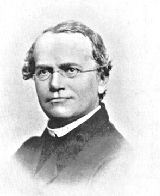
\includegraphics{figs/mendel1862.jpg}}\\
\small Gregor Mendel\\ (1822--1884)\\
(\small \href{http://commons.wikimedia.org/wiki/File:Mendel.png}{Image source})
} Although Mendel published his work in 1866 it was not widely noticed until around 1900, and not until the 1930's was Mendelian genetics fully integrated into evolutionary theory (the so-called ``Modern Synthesis''). This led to the creation of the new science of population genetics which now forms the theoretical basis for all evolutionary biology. 



\section{Mendelian Genetics}

I will here briefly summarize some important aspects of Mendelian genetics\index{Mendelian genetics}, and present a number of definitions that will be used later in the text. 
\begin{figure}[!t]
\begin{center}
\resizebox{\textwidth}{!}{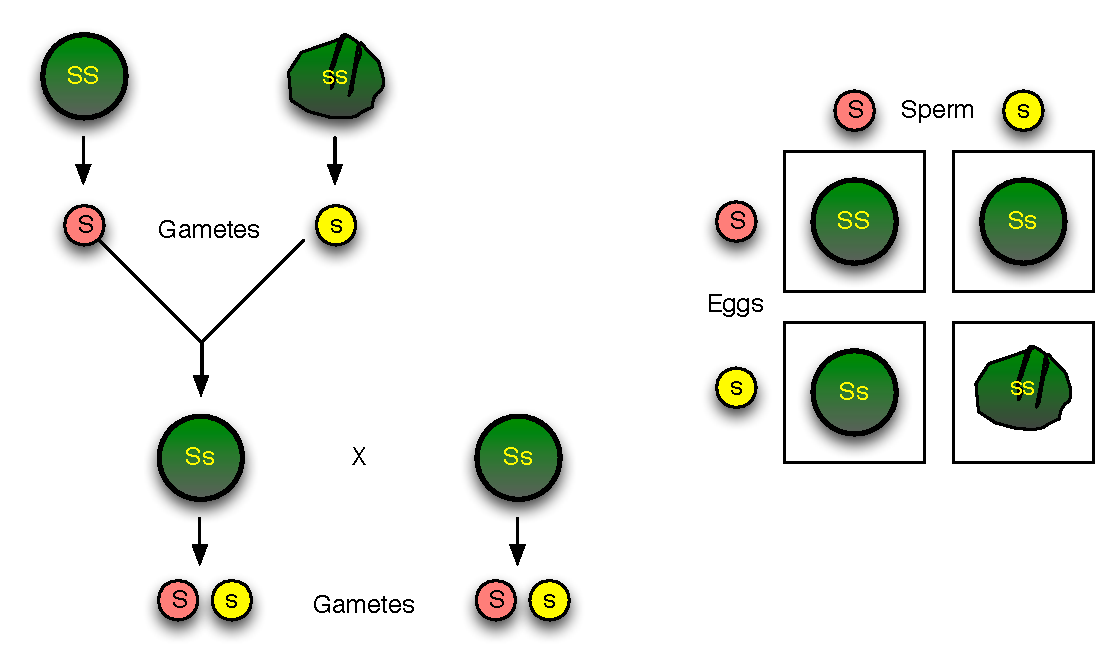
\includegraphics{figs/mendeliangenetics.pdf}}
\caption{\small Mendelian genetics. Each diploid parent pea contains two alleles. The s allele is recessive and results in wrinkled peas when present in two copies.}
\label{alleles}
\end{center}
\end{figure}

An organism can be either haploid or  diploid. {\bf  Haploid}\index{Haploid} organisms have one complete set of genetic material (and therefore one copy of each gene), while {\bf diploid}\index{Diploid} organisms have two  complete sets of genetic material located on two complete sets of chromosomes (and therefore two copies of each gene). A particular gene in a haploid or diploid organism is said to occupy a particular {\bf locus}\index{Locus} (plural: loci). If different versions of a gene are present at a particular locus (\eg in different individuals of a population) then these are referred to as {\bf alleles}\index{Allele} of that gene. A diploid organism may have different alleles present on the two individual copies of a chromosome. If a diploid organism has the same allele on both chromosomal copies, then it is said to be {\bf homozygous}\index{Homozygous} for that allele (it is a homozygote). If it has two different alleles present at a locus, then it is said to be {\bf heterozygous}\index{Heterozygous} for that allele (and is then referred to as a heterozygote). The total complement of alleles present in an organism is its {\bf genotype}\index{Genotype}.  If we are interested in one particular locus where the alleles $A$ and $a$ occur, then a diploid organism might for instance have the genotype ``$AA$'' or ``$Aa$''. A haploid organism might have the genotype ``$a$'' at such a locus. Depending on the molecular nature of the different alleles present at a locus in a diploid organism, one allele may not make an impact on the organisms appearance (its {\bf phenotype}\index{Phenotype}). It is then said to be a {\bf recessive}\index{Recessive} allele. An allele that is fully expressed in the organism's phenotype is called {\bf dominant}\index{Dominant}. For instance,  Fig. \ref{alleles} shows two different alleles---the dominant $S$ allele and the recessive $s$ allele---of a gene controlling wrinkledness in peas. Occasionally the alleles will be co-dominant, and this will result in an apparent blending of parental characteristics. In diploid organisms, one allele comes from the mother, one from the father. When diploid organisms reproduce sexually, it occurs via an intermediate, haploid sex cell called a  {\bf gamete}\index{Gamete} (the gamete is an egg cell if it is produced by a female, and a sperm cell if it is produced by a male). During gamete formation, genetic material from the two parents is mixed by the process of {\bf recombination}. Recombination is one stage of the special type of cell division termed {\bf meiosis}\index{Meiosis} which ultimately results in formation of the haploid gamete. At any one locus, there will (by necessity) be only one allele present in the gamete. The diploid cell formed by fusion of two gametes is called a {\bf zygote}\index{Zygote}. Sexually reproducing\index{Sexual reproduction} organisms have life cycles that alter between a haploid stage and a diploid stage. In some organisms most of the life cycle is diploid (\eg humans, where only the sex cells are haploid), while the situation is reversed for other organisms (including some algae where the diploid zygote quickly undergoes meiosis to form new haploid cells). There are also organisms (\eg ferns) where the life cycle alternates between a haploid, multicellular generation and a diploid, multicellular generation. Asexual reproduction\index{Asexual reproduction} is seen in both haploid organisms (\eg bacteria) and diploid organisms (\eg yeast and some plants). 

%%%%%%%%%%%%%%%%%%%%%%%%%%%%%%%%%%%%%%%%%%%%%
%							CHAPTER
%%%%%%%%%%%%%%%%%%%%%%%%%%%%%%%%%%%%%%%%%%%%%

\chapter{Brief Introduction to Population Genetics}
		\fancyhead[LO]{Chapter 2: Brief Introduction to Population Genetics}		
		\fancyhead[RE]{Molecular Evolution, lecture notes}
		\fancyfoot[LO,RE]{\footnotesize  \  Anders Gorm Pedersen, \the\year{}}
		\clearpage

\section{Introduction}

The science of population genetics deals with genetic variation within populations, and with the forces that change this variation. I will now give you a very brief introduction to a few important results in the field. 

My goal with this section is mostly to make you aware of some of the ways in which evolutionary theory can be approached in a stringent, quantitative manner.  Specifically, we will discuss the effects that growth, selection, mutation, and genetic drift have on the genetic composition of a population. Most of the concepts will be introduced in the context of haploid, asexually reproducing organisms since that makes the analysis easier.

The material covered here does not \emph{directly} relate to reconstruction of phylogenetic trees. However, any evolutionary history is necessarily the result of processes that resemble the ones described in this section, and it is therefore relevant to have at least passing knowledge of the underlying theory. 
%
%Population genetics \emph{does} rely rather heavily on the use of algebra. However, I have attempted to explain every single step carefully, and it is my hope that everyone should be able to follow the derivations. In fact, one of my goals with this course is to eliminate any trace of math-anxiety you may have (which is useful if you want to understand the technical details of, for instance, maximum likelihood phylogenetic reconstruction). Of course, some of you might find the math entirely trivial, but the opposite seems to be the norm among students of biology (I know that's how I feel most of the time). 

\section{Population Growth}
\subsection{Exponential Growth}

We will start by analyzing the characteristics of a growing population. Imagine that we are examining a population of asexually reproducing organisms where each individual produces 200 offspring per generation and then dies. The number $200$ is called the fecundity\index{Fecundity} of the organism and is usually denoted $m$. For various reasons only $2\%$ of the offspring survive sufficiently long to produce offspring of their own. This is the survival rate and is usually denoted $L$. We can easily see that each individual organism will have a net life-time production of $m\times L=200\times~2\%=4$ descendants. This number is the so-called per capita reproductive rate\index{Reproductive rate} ($R$) of the population. It is also clear that since each individual leaves more than one descendant, then the population will grow. But how exactly will that growth proceed? 

Let us first assume that the numbers $L$ and $m$ remain constant in subsequent generations, and that generations are discrete and non-overlapping. This means that for every organism that was present at some point in time, there will be $R$ individuals present after one generation ($4$ in the example above). Thus, the population size after one generation~($N_1$) can be computed from the initial population size~($N_0$) as follows:
%
\begin{equation*}
\label{}
N_1=N_0\times R
\end{equation*}
%
The population size after two generations can be found by multiplying this number by $R$ one additional time, and we therefore have:
%
\begin{align*}
\notag N_2 &=N_1\times R\\
\notag	&=N_0 \times R\times R\\
	&= N_0\times R^2
\end{align*}
%
More generally, after $t$ generations we have that
%
\begin{equation}
\label{EQexpgrowth}
N_t=N_0 R^t
\end{equation}
%
\begin{figure}[!t]
\begin{center}
\resizebox{\textwidth}{!}{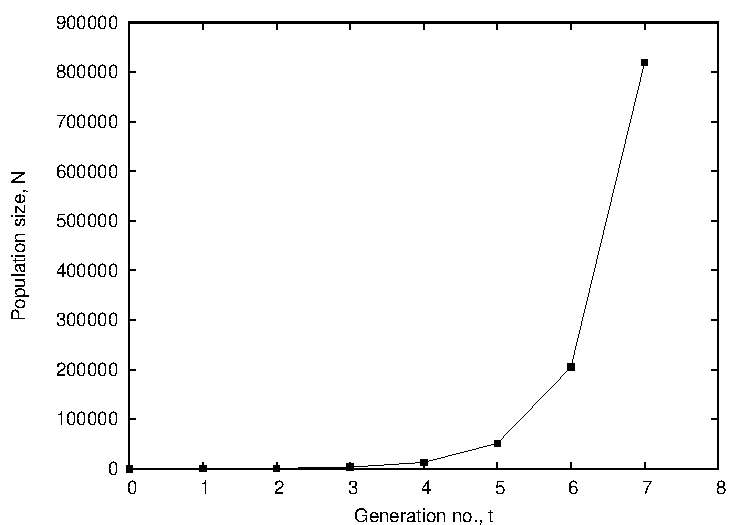
\includegraphics{figs/expgrowth.pdf}}
\caption{\small Exponential growth with discrete, non-overlapping generations. The plot shows the growth of a population with initial size $N_0=50$ and per capita reproductive rate $R=4$.}
\label{FIGexpgrowth}
\end{center}
\end{figure}
%
This type of relationship is called exponential growth\index{Exponential growth}. Figure \ref{FIGexpgrowth} shows how the population size will increase for a population with $R=4$ and $N_0=50$. After only 7 generations the population size has increased to more than 800,000. Note that $R$ gives the rate of increase \emph{per generation}, and $t$ therefore has to be measured in \emph{generations}. Moreover, $t$ can only be changed in discrete steps of one full generation, giving the discontinuous curve seen above.
%
\begin{figure}[!t]
\begin{center}
\resizebox{\textwidth}{!}{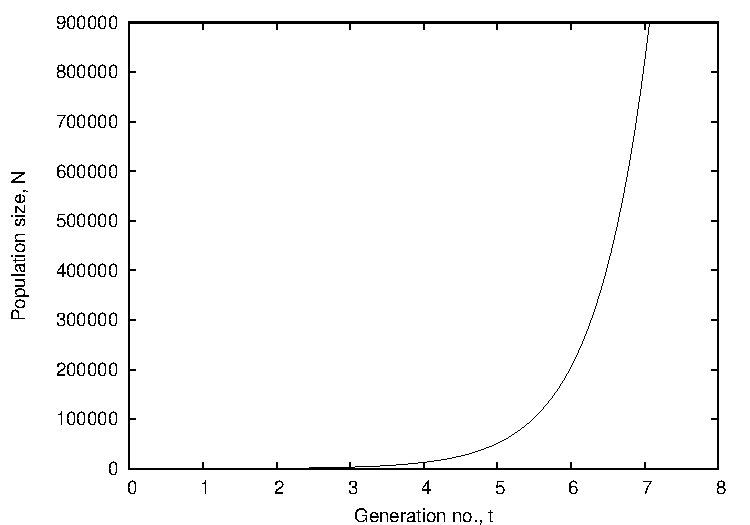
\includegraphics{figs/expgrowthcont.pdf}}
\caption{\small Exponential growth with continuous reproduction and/or overlapping generations. The plot shows the growth of a population with initial size $N_0=50$ and instantaneous rate of increase $r=1.39$ per generation (corresponding to a per capita reproductive rate $R=4$).}
\label{FIGcontexpgrowth}
\end{center}
\end{figure}
%
%The model developed here is as far as we will explore population growth in any detail. I will briefly mention %more advanced models, but it is not important that you understand the details of these.

The exponential growth model derived here assumes that generations are discrete and non-overlap\-ping. Typically, however, individuals do not breed synchronously. Furthermore, it is often the case that offspring is produced not only once but several times during the life-span of an organism. Accounting for the phenomena of continuous reproduction and overlapping generations, requires slightly more complicated derivations but leads to models that are very similar to the one above. Without going into the details, we may note that the growth in such situations can be described by the following expression:
%
\begin{equation}
\label{ }
N_t = N_0  e^{rt}
\end{equation}
%
Since births can now take place at any given time, the variable $t$ can here take on any real value (not just integers). Furthermore, $t$ can now be expressed in any unit of time (hours, days, years, generations, \etc). An example of continuous exponential growth is shown in figure \ref{FIGcontexpgrowth}. 

The constant $r$ is called the ``instantaneous rate of increase'' and has to be expressed in units that match those of $t$ (if $t$ is measured in minutes, then~$r$ has to be measured in ``per minute''.) If $r$ is expressed in units of ``per generation'', then the per capita life-time rate of increase $R$ can be found by: $R=e^r$.\\
\\
%is that true?

%\begin{exercise}
%\label{Xcoliearth}
{\bf Exercise 2-1: }
The bacterium \emph{Escherichia coli} has a generation time of about $20$ minutes when growing in rich medium (\ie $R=2$, one generation time corresponds to $20$ minutes). The weight of a single \emph{E. coli} cell is approximately $1\times 10^{-12}$g . The weight of planet earth is approximately $6 \times 10^{24}$kg $= 6\times 10^{27}$g. Calculate how long it will take for a population of 100 \emph{E. coli}  cells to grow to the point where the combined weight of the bacteria is the same as the weight of the earth. Use the fact that equation  \ref{EQexpgrowth} can be rearranged to give:

\begin{equation*}
t = \frac{\log{\tfrac{N_t}{N_0}}}{\log{R}} \label{texp}
\end{equation*}

%\answer
%No. of coli cells required to weigh as much as the earth: $N_t = \frac{6\times 10^{27}g}{10^{-12}g/cell} = 6\times 10^{39}$ cells. This gives $t=\frac{\log{\tfrac{N_t}{N_0}}}{\log{R_m}}=\frac{\log{\tfrac{10^{39}}{100}}}{\log{2}}=125$ generations, corresponding to $125\times 20 minutes=2500 minutes=41 hours$

%\end{exercise}

\subsection{Logistic Growth}

As illustrated by exercise 2-1 the exponential growth model is over-simplified in that growth will normally be limited by the finite resources available (food, space, \e{etc}.).  Exponential growth is therefore only seen for limited amounts of time and under special circumstances. Examples include the initial growth of bacterial cells in test tubes and the growth of larger organisms after entering an unoccupied ecological niche. The so-called logistic growth model attempts to capture these limits to growth by having the rate of increase depend on the population size (the rate drops as the population size increases). Under this model, the population size will eventually reach a plateau referred to as the ``carrying capacity'' and usually denoted $K$. Logistic growth may be described by the following expression:
%
\begin{equation}
\label{EQlogisticgrowth }
N_t = \frac{K}{1+ \left( \frac{K}{N_0}-1\right)e^{-rt}}
\end{equation}
%
An example of logistic growth with carrying capacity $K=10,000$, rate of increase $r=1.1$, and initial population size $N_0=100$, is shown in Fig. \ref{FIGlogistic}. Note how the population size initially seems to grow exponentially, but subsequently levels off, finally converging on the carrying capacity. The logistic growth model may be modified further to account for situations where the effect of population size on the growth rate is not instantaneous but has a time lag. 
%
\begin{figure}[!t]
\begin{center}
\resizebox{\textwidth}{!}{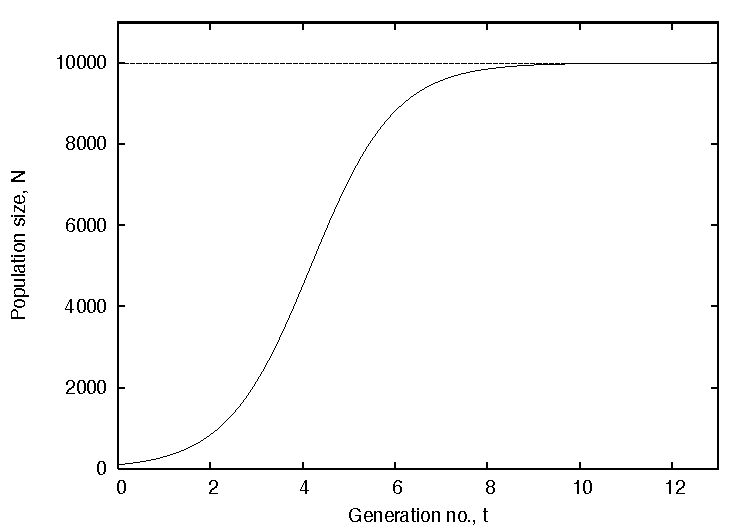
\includegraphics{figs/logistic.pdf}}
\caption{\small Logistic growth. The plot shows the growth of a population with initial size $N_0=100$, rate of increase $r=1.1$, and carrying capacity $K=10,000$.}
\label{FIGlogistic}
\end{center}
\end{figure}
%

\section{Genotype Frequencies and Growth\label{SECfreqgrowth}}

Above, we have started developing an understanding for how populations grow. We will now move on to investigate what happens when a growing population consists of a number of distinct genotypes.  Let us first consider the fate of two different alleles---$A$ and $a$---that are present in a population of haploid, asexually reproducing, exponentially growing organisms with discrete, non-overlapping generations (\ie a population whose growth is described by the equation $N_t=N_0*R^t$). The allele $A$ is present in a fraction $f_A$ of all individuals at the time we start our examination. The other allele, $a$, is present in the remaining fraction $f_a$. Note that $f_A+f_a=1$. If we denote the initial (total) population size by $N_0$, then the initial number of individuals with alleles $A$ and $a$ are: 
%
\begin{align*}
N_{A,0} &= f_A  N_0\\
N_{a,0} &= f_a N_0
\end{align*}
%
We again assume that the average, per capita reproductive rate ($R$) of the entire population remains constant in subsequent generations. We furthermore assume that the two \e{genotypes} have the same growth rate (Thus, $R_A=R_a=R$). The average, per capita life-time reproductive rate of a genotype is also referred to as that genotype's ``absolute fitness''\index{Fitness!absolute}. From equation \ref{EQexpgrowth} we have the following expressions for the number of individuals with genotypes $A$ and $a$ after one generation:
%
\begin{align*}
N_{A,1} &= N_{A,0} R = f_A  N_0  R\\
N_{a,1} &= N_{a,0} R = f_a N_0 R
\end{align*}
%
The total population size after  one generation will therefore be 
%
\begin{align*}
N_1 &= N_{A,1} + N_{a,1} \\
	&=  f_A  N_0  R + f_a N_0 R\\
	&= N_0 R \times (f_A + f_a)\\
	&= N_0 R
\end{align*}
(since $f_A+f_a=1$). We can now compute the frequency of individuals with genotype $A$ after one generation:
%
\begin{equation*}
f_{A,1} = \frac{N_{A,1}}{N_1} = \frac{f_A N_0 R}{N_0 R} = f_A\\
\end{equation*}

The frequency of individuals with genotype $A$ after one generation of growth ($f_{A,1}$) is therefore the same as the frequency of $A$ at the outset ($f_A$), and we can conclude that if different genotypes have the same reproductive rate, then their proportions are not changed by asexual reproduction. (The same is obviously true for allele $a$).

Note that this result holds regardless of whether the population size is increasing (corresponding to $R > 1$) or decreasing (corresponding to $R<1$), as long as the different genotypes have the same absolute fitness,~$R$. (If the two genotypes do \e{not} have the same absolute fitness then there is natural selection for the genotype with the higher value. We will return to that situation below).  Importantly, constancy of genotype frequencies during growth will be true for any type of organism with asexual reproduction, regardless of whether the organism is haploid or diploid. In the latter case $f_A$ would refer to the frequency of a given \e{diploid} genotype. If all diploid genotypes ($AA$, $aa$, and $Aa$) retain their initial frequencies, then the frequency of any single allele ($A$ and $a$) will again remain unchanged.

In this section, we have ignored the statistical uncertainty that will play a role for small populations. We will return to chance effects and the phenomenon of ``genetic drift'' in section \ref{SECdrift}.

\section{Selection \label{SECselection}}

Let us now consider the more interesting case where two haploid genotypes do \e{not} have the same absolute fitness. We will again investigate an example where the alleles $A$ and $a$ are present at a locus in a haploid organism that reproduces as described above. Let us imagine that the absolute fitness of genotype $A$ is $R_A=4$, while that of genotype $a$ is $R_a=2$. Recall that for organisms such as the one we are examining here, $R$ is the product of fecundity and survival rate. It is therefore possible that the difference in fitness between the two genotypes is caused by differential fecundity, differential survival rate, or both. Let us say, for instance, that genotype $A$ has a fecundity of 200 offspring per generation, and a survival rate of 2\%, giving $R_A=200\times 2\%=4$. We may further imagine that genotype $a$ has a higher fecundity (400 offspring per generation) but a much lower survival rate (0.5\%) resulting in an overall fitness that is half that of genotype $A$ ($R_a=400\times 0.5\%=2$). 

\begin{figure}[!t]
\begin{center}
\resizebox{\textwidth}{!}{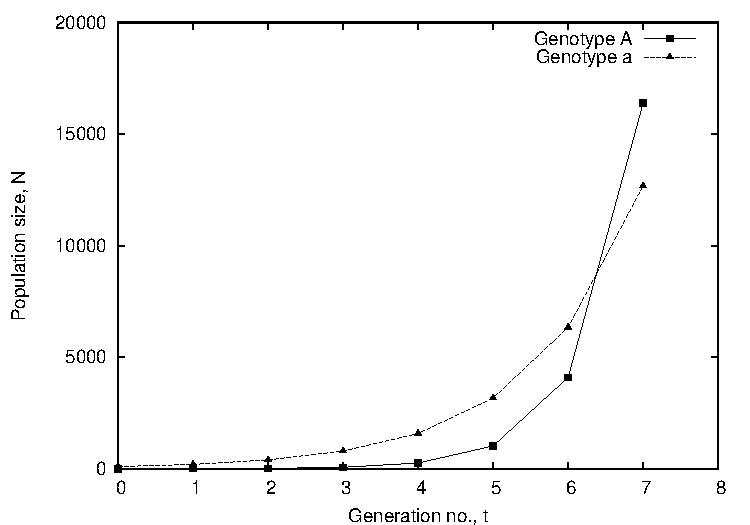
\includegraphics{figs/natsel.pdf}}
\caption{\small Natural selection in haploid organisms. Genotype $A$ (initial number $N_{A,0}=1$) has the fitness $R_A=4$, while genotype $a$ ($N_{a,0}=99$) has a lower fitness ($R_a=2$). Differential exponential growth of two genotypes is one instance of natural selection}
\label{FIGnatsel}
\end{center}
\end{figure}

The number of individuals with genotype $A$ therefore grows faster than the number of individuals with genotype $a$. An example of this is shown in Figure \ref{FIGnatsel}. Table \ref{TABnatsel} gives the corresponding genotype numbers and frequencies,  and includes a few extra generations compared to the figure. In this example, the initial population consists of one single individual with genotype $A$ (perhaps a newly created mutation), and 99 individuals with genotype $a$. It can be seen how the proportion of individuals with genotype $A$ rapidly increases from the initial 1\%, and after 7 generations $A$ is the predominant genotype. After only 10 generations genotype $A$ makes up more than 90\% of the population, and intuitively it seems to be approaching 100\% asymptotically (Table \ref{TABnatsel}). But instead of guessing, we should of course develop a  mathematical model that we can use to predict the genotype frequencies at any time $t$. 


Let us again define the initial frequencies of individuals with genotypes $A$ and $a$ to be  $f_A$ and $f_a$ respectively ($f_A+f_a=1$), and denote the initial total population size $N_0$. We therefore have the following numbers of individuals with $A$ and $a$ at the time we start:
%
\begin{align*}
N_{A,0} &= f_A N_0\\
N_{a,0} &= f_a N_0
\end{align*}
%
After $t$ generations we have the following numbers:
%
\begin{align*}
N_{A,t} &= N_{A,0}(R_A)^t = f_A N_0 (R_A)^t\\
N_{a,t} &= N_{a,0}(R_a)^t = f_a N_0 (R_a)^t
\end{align*}
%
\begin{table}[!t]
\footnotesize
\caption{\small Differential growth. $f_A$: freq. of genotype $A$, $f_a$: freq. of genotype $a$.}
\begin{center}
% the tabular* environment allows to define table width, but in order to get the columns spread out,
% there also needs to be expanndable space (rubber space) between columns.  That's what extracolsep does
\begin{tabular*}{\textwidth}{@{\extracolsep{\fill}}crrrcc}
\hline 
$t$ 	& $N_A$ &  $N_a$ & $N_{tot}$ & $f_A$  & $f_a$\\
\hline 
0 &	1		&	99		& 	100 		&	0.01	&	0.99\\
1 &	4		&	198		& 	202 		&	0.02	&	0.98\\
2 &	16		&	396		&	412 		&	0.04	&	0.96\\
3 &	64		&	792		&	856 		&	0.07	&	0.93\\
4 &	256		&	1584		&	1841		&	0.14	&	0.86\\
5 &	1024		&	3168		&	4192		&	0.24	&	0.76\\
6 &	4096		&	6336		&	10432	&	0.39	&	0.61\\
7 &	16384	&	12672	&	29056	&	0.56	&	0.44\\
8 &   65536	&	25344	&	90880	&	0.72	&	0.28\\
9 &   262144	&	50688	&	312832	&	0.84	&	0.16\\
10 &	1048576	&	101376	&	1149952	&	0.91	&	0.09\\
%11 &	4194304	&	202752	&	4397056	&	95	&	5\\
\hline 
\end{tabular*}
\end{center}
\label{TABnatsel}
\end{table}%
%
Therefore the total population size at time $t$ will be:
\begin{equation*}
N_{\text{tot},t} = N_{A,t} + N_{a,t} = f_A N_0 (R_A)^t + f_a N_0 (R_a)^t
\end{equation*}
The \e{frequency} of individuals with genotype $A$ after $t$ generations is therefore:
%
\begin{equation*}
\label{EQseltmpres}
f_{A,t} = \frac{N_{A,t}}{N_{\text{tot},t}} =\frac{f_A N_0 (R_A)^t}{f_A N_0 (R_A)^t + f_a N_0 (R_a)^t} =\frac{f_A (R_A)^t}{f_A (R_A)^t + f_a (R_a)^t} 
\end{equation*}
%
Where the last simplification was obtained by eliminating $N_0$. The expression can be further simplified by dividing both the numerator and the denominator with $(R_A)^t$:
%
\begin{equation}
\label{EQselalmostdone}
f_{A,t} = \frac{f_A (R_A)^t\times \frac{1}{(R_A)^t}}{(f_A (R_A)^t + f_a (R_a)^t)\times \frac{1}{(R_A)^t}}  = \frac{f_A}{f_A+f_a\frac{(R_a)^t}{(R_A)^t}} =  \frac{f_A}{f_A+f_a(\frac{R_a}{R_A})^t}
\end{equation}
%
The term $\frac{R_a}{R_A}$ is the so-called ``relative fitness''\index{Fitness!relative} of allele $a$. The relative fitness of a genotype (usually denoted $W$) is the fitness of that genotype relative to a reference genotype (typically the genotype with the highest fitness). In our example we therefore have that $W_a = \frac{R_a}{R_A} = \frac{2}{4} = 0.5$, and $W_A = \frac{R_A}{R_A} = 1$. Substituting $W_a$ for $\frac{R_a}{R_A}$ in equation \ref{EQselalmostdone}, we get:
%
\begin{equation}
\label{EQselproof}
f_{A,t} = \frac{f_A}{f_A + f_a W_a^t}
\end{equation}
%
And here, finally, is our result: equation \ref{EQselproof} enables us to compute how natural selection changes the frequencies of genotypes $A$ and $a$ over time (The frequency of genotype $a$ can, for instance, be found by $f_{a,t} = 1-f_{A,t}$.) An important conclusion from equation \ref{EQselproof} is that the effect of natural selection only depends on the \e{relative} fitness. This means that we would get the same change in frequency regardless of whether the absolute fitnesses of $A$ and $a$ were, for instance, 10 and 5, or 6 and 3, or even 0.8 and 0.4 respectively. 

\begin{figure}[!t]
\begin{center}
\resizebox{\textwidth}{!}{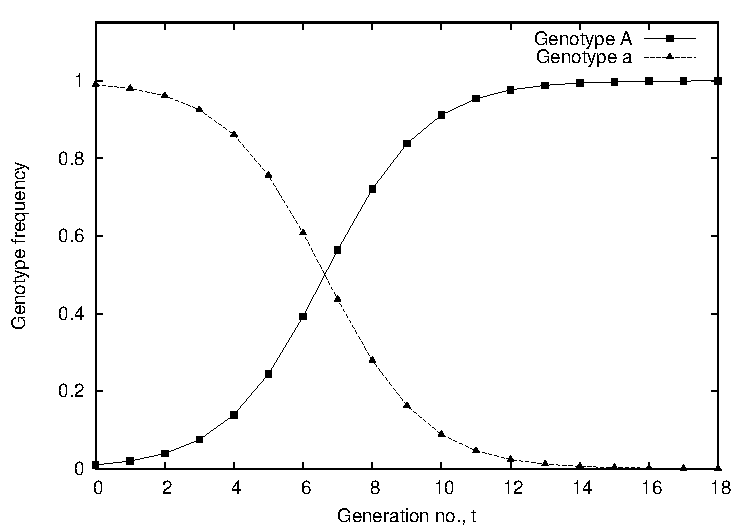
\includegraphics{figs/natselproof.pdf}}
\caption{\small Change in genotype frequencies as a result of natural selection. Genotype $A$ (initial number $N_{A,0}=1$) has the fitness $R_A=4$, while genotype $a$ ($N_{a,0}=99$) has a lower fitness ($R_a=2$).}
\label{FIGnatselproof}
\end{center}
\end{figure}


The so-called selection coefficient ($s$) is often used instead of the relative fitness $W$. The selection coefficient against the least fit allele is defined as $s=1-W$ where $W$ is the relative fitness of the least fit allele. This means that $W=1-s$ and equation \ref{EQselproof} can of course be rewritten by substituting $(1-s)$ for $W_a$, if one is interested in expressing the frequencies in terms of selection coefficients instead of relative fitness. 


Figure \ref{FIGnatselproof} shows how the genotype frequencies change over time in our example  (\ie when $W_a=0.5$). A relative fitness of $0.5$ corresponds to a selection coefficient of $s=1-0.5=0.5$. It can be seen that even though genotype $A$ has an initial frequency of only 1\%, it has essentially reached fixation after just 16 generations. It should be noted that a selection coefficient of $0.5$ is quite high, but it is not unrealistic. For instance it has been estimated that natural selection acting on the so-called melanic peppered moths, that spread in industrial Britain during the 1800's, involved a selection coefficient of approximately $0.3$. It is believed that this selection was driven by the dark, melanic forms being harder to detect on soot-covered tree bark compared to the lighter, more easily spotted form of the moth. Selection for drug resistance in HIV and pesticide resistance in mosquitoes has also been reported to be of this magnitude. 

Figure \ref{FIGnatsel2} shows another example where the $a$ allele has a relative fitness of 0.99 (corresponding to a selection coefficient $s=0.01$). In this example genotype $A$ has essentially reached  fixation after 1000 generations. It is important to note that there are situations where natural selection will not lead to fixation of one allele, but will instead act to maintain a certain level of diversity at a locus. One example of this is when a diploid organism that is heterozygous at some locus has higher fitness then either of the two homozygotes. 

\begin{figure}[!t]
\begin{center}
\resizebox{\textwidth}{!}{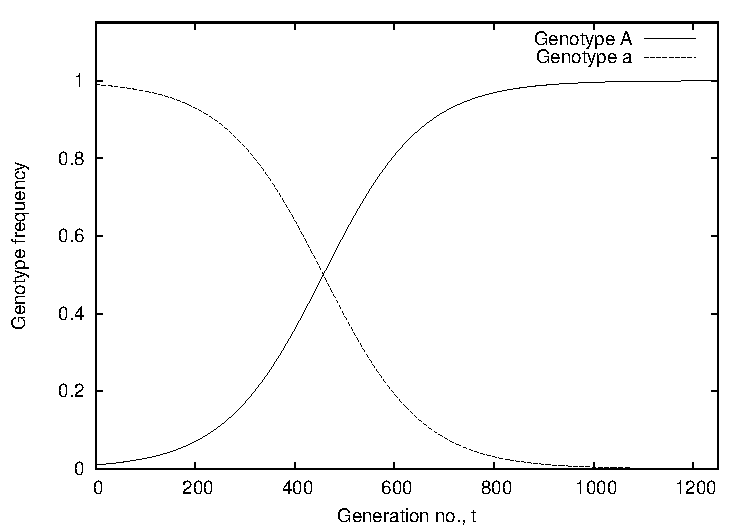
\includegraphics{figs/natselproof2.pdf}}
\caption{\small Change in genotype frequencies as a result of natural selection. Relative fitness of genotype $a$ is $0.99$ corresponding to a selection coefficient of $s=0.01$}
\label{FIGnatsel2}
\end{center}
\end{figure}

\section{Mutation-Selection Balance\label{SECmutselbal}}

\index{Mutation-selection balance}\index{Selection-mutation balance}
The model of selection developed above, shows how an advantageous allele ($A$) will spread through a population and eventually reach fixation. Similarly, selection will act to eliminate the disadvantageous allele ($a$) from a population. But what if the disadvantageous allele is constantly being produced at some rate by mutation?  In that case selection cannot remove the allele entirely and instead its frequency will eventually reach a constant equilibrium value. (If the frequency of the disadvantageous allele falls beneath the equilibrium value then mutation will act to increase it again. If the frequency of the disadvantageous  allele becomes too high, then natural selection will lower it). We are interested in computing the equilibrium  frequency. 

Let us again consider a haploid, asexual organism where we are examining the two alleles $A$ and $a$, and  where genotype $a$ has a lower fitness than genotype $A$.  For instance, genotype $a$ may  have a relative fitness of $W_a=0.95$  corresponding to a selection coefficient $s=0.05$. Now, let us also imagine that allele $A$ mutates to allele $a$ with mutation rate $m$ (we can imagine, for instance, that $A$ corresponds to a functional enzyme while $a$ refers to all non-functional forms of the enzyme). Let us set $m=10^{-7}$ mutations per $A$-gene per generation. This is a fairly typical mutation rate for a gene, and  means that in any one generation $\frac{1}{10,000,000}$ of all $A$-alleles will mutate to an $a$-allele. 

We will now derive an expression that gives us the frequency of the disadvantageous allele $a$ at equilibrium. We will do this by first considering how the forces of mutation and selection combine to change the frequency of $A$ during one single generation. To simplify matters, we will assume that the effects of selection and mutation act sequentially\footnote{This derivation follows Felsenstein. See \url{http://evolution.genetics.washington.edu/pgbook/pgbook.html}}:
\begin{equation*}
\text{G1} \quad (p) \quad \xrightarrow[\text{selection}]{}\quad  \text{G2} \quad (p^*) \quad  \xrightarrow[\text{mutation}]{}\quad  \text{G2} \quad (p_1)\quad \xrightarrow[\hspace{10mm}]{}\quad ...
\end{equation*}
%
Here, $p$ is the frequency of $A$ in generation 1 organisms just prior to reproduction; $p^*$ is the increased frequency of $A$ in generation 2 after selection has acted (via fecundity and survival rate); $p_1$ is the final frequency of $A$ in adult generation 2 organisms after one full life-cycle has elapsed, and mutation has decreased the frequency of $A$ (thereby producing more $a$). 

To find the equilibrium value, you should first recall that equation \ref{EQprecurrence} (page \pageref{EQprecurrence}) tells us that the natural selection step will change the frequency of genotype $A$ as follows:
%
\begin{equation}
\label{EQAincrate}
p^*= \frac{p}{1-sq}
\end{equation}
%
We now need to figure out how the mutation step will change this frequency. Note that the mutation rate $m$ gives the fraction of $A$ alleles that will change into $a$ in the course of one generation. The fraction of $A$ individuals that \e{remain} $A$ must therefore be $1-m$ and we consequently have that:
%
\begin{equation*}
\notag  p_1 = p^*(1-m)
\end{equation*}
%
Substituting the expression in equation \ref{EQAincrate} for $p^*$  gives us:
%
\begin{equation}
\label{EQtmpmutsel}
p_1 = \frac{p(1-m)}{1-sq}
\end{equation}
%
This expression tells us how the forces of selection and mutation combine to change the frequency of $A$ (from $p$ to $p_1$) in one generation. We can now find the equilibrium frequency by using the following insight: at equilibrium the frequency of $A$ is constant. From this it follows that the frequency of $A$ after one generation ($p_1$) must equal the frequency of $A$ in the previous life-cycle ($p$). Substituting $p$ for $p_1$ in equation \ref{EQtmpmutsel} gives us:
%
\begin{equation*}
p = \frac{p(1-m)}{1-sq}
\end{equation*}
%
Multiplying either side of this equation by $(1-sq)$ gives us
%
\begin{equation*}
p(1-sq)  = p(1-m)
\end{equation*}
We can now eliminate $p$ from this equation and isolate the equilibrium frequency of $a$:
\begin{align}
\notag 1-sq &= 1-m \\[3mm]
\notag sq &=m \\[3mm]
q &=\frac{m}{s} \label{EQmutsel}
\end{align}
%
Equation \ref{EQmutsel} shows us that the equilibrium frequency of the disadvantageous allele depends on only the mutation rate and the selection coefficient in a very simple way. In our example we  find that the equilibrium frequency of $a$ is:
%
\begin{equation*}
q=\frac{m}{s} = \frac{10^{-7}}{0.05} = 2 \times 10^{-6}
\end{equation*}

The conclusion from the analysis presented here,  is that when both selection and mutation are acting at the same time, then a constant and predictable level of genetic diversity will be maintained in the population. 

\section{Mathematical Modeling: A Few Thoughts\label{SUBSECmathmodel}}

The science of population genetics deals with understanding the genetic variation within populations, and the forces that change this variation.  The use of mathematical models is important in this field. Mathematical modeling will also play an important role later in this course when we discuss phylogenetic reconstruction and it is therefore relevant at this point to briefly consider the subject\index{Modeling!mathematical}. First, I would like to make two important points about the nature of models:\\

\begin{enumerate}

\item {\bf A mathematical model is an explicitly stated hypothesis}

A mathematical model that describes a biological system can be thought of as a very explicitly and stringently  phrased hypothesis about how that system works. The explicitness of a hypothesis stated this way, means that it is possible to make very detailed predictions about how the investigated system will behave under different conditions. As is the case for predictions based on qualitative hypotheses, such quantitative predictions can be checked against real world data, and the model modified or abandoned for a more suitable model if necessary.

\item {\bf A mathematical model does not represent full reality}

It is typically not possible to represent full reality in a mathematical model. For instance, even the intuitively reasonable growth models considered above, assumed that there was a well defined (and constant) average fitness for a given genotype. In reality, both fecundity and survival rate depend on a large number of interacting biological and non-biological, internal and external factors for each individual in the population. Some of these factors will be stochastic (falling trees, heart attacks, infection, \emph{etc.}). To approach full reality in the model we would therefore need to model fecundity and survival rate of all individuals, and for each individual these would be complicated functions of huge numbers of different terms. It should be clear that for most biological systems, representing full reality in a mathematical model is impossible. Fortunately, that's not something we are interested in doing in the first place! For a typical biological system, we will instead be more interested in finding an approximating model that captures the most important features, and allowing us to understand the dynamics of the system.

\end{enumerate}


\section{Genetic Drift \label{SECdrift}}\index{Genetic drift}\index{Drift}

In the discussion presented above we have been using models  that are ``deterministic''. Deterministic models\index{Model!deterministic} are characterized by always giving a specific result when starting from a specific set of conditions. For instance, when we investigated exponential growth above, it was assumed that if a population has growth rate  $R=4$ and initially consists of $N_0$ individuals, then there will be  \e{exactly} $4\times N_0$ individuals in the next generation. Based on this assumption we showed that the proportions of different genotypes will remain constant  provided that the genotypes have the same fitness (section \ref{SECfreqgrowth}). 

This is, however, a simplification. Different individuals will not leave \e{exactly} the same number of offspring, and death will also not remove \e{exactly} the same fraction of different broods. This means that for every generation there is some chance that the frequency of a genotype will change, even though it has the same fitness as all other alleles at the locus (alleles with the same fitness are said to be ``neutral''). 

The frequency of an allele has an equal chance of changing to a higher or a lower value. This is true for every consecutive generation, regardless of what the frequency has been at any previous time. Imagine for instance that an allele has changed from its initial value of $p=0.3$ to $p=0.26$. In the next generation the chance of ending with a frequency that is higher than  $0.26$ will be the same as the chance of ending with  a frequency that is lower than $0.26$. If, after $100$ generations, the frequency has changed to $0.0001$, then there  will still be the same chance for the frequency to either increase or decrease in the next generation.  If this fluctuation continues for sufficiently long then $p$ will eventually wander to either $0$ or $1$.  Once that has happened the allele frequency can no longer change (at least if we assume that there is no mutation and no migration from other populations). 

The process of random change in genotype frequencies is called genetic drift. From the discussion above, it can be seen that genetic drift (on its own) tends to reduce the level of genetic variation in a population. This is similar to the effects of selection described in section \ref{SECselection}, but in the case of fixation by drift, the fixed allele will not be advantageous compared to the lost alleles. In fact, fixation will  be the result of entirely random processes, and different alleles will be fixed in different populations. The DNA sequences in isolated populations will therefore tend to drift apart over time. 

\section{Chance of Fixation by Drift}

We will consider the fate of individual genes in a population of haploid, asexually reproducing organisms subject to only genetic drift. Let us assume that the number of individuals ($N$) is constant. For instance, we can imagine that the average  fecundity is $200$ and the average  survival rate $\frac{1}{200}$, meaning that each individual leaves one offspring per generation. This is only the average however. Some individuals will leave no offspring, some will leave one, and some will leave two or more, resulting in a gradual change in genotype frequencies by genetic drift. Let us further imagine that every individual in the population initially has a distinct genotype ($A_1, A_2, \cdots, A_N$). The  frequency of each genotype is therefore initially $\frac{1}{N}$. According to the argument above, one of the individual genes in the population will eventually reach fixation. Since this process is entirely random the different alleles must all have the same chance of fixation, and we can conclude that the chance that any particular allele ($A_5$ for instance) is fixed, must be $\frac{1}{N}$. Similarly, if an allele is initially present in $x$ copies, then it has the probability $\frac{x}{N}$ of eventually being fixed (since each of the $x$ copies have probability $\frac{1}{N}$ of being fixed). Generally, the probability that an allele $A_i$ will be fixed  is the same as the frequency $f_i$ of that allele . 

\section{Drift and Neutral  Mutation\label{SECdriftmut}}

Genetic drift ultimately results in the loss of genetic diversity, but since this loss is the result of random fluctuations, drift is not a particularly strong or fast-acting evolutionary force. It can be shown that, on average, it takes $2N$ generations for a new mutation to reach fixation in a haploid, asexually reproducing population of $N$ individuals.  The process takes $4N$ generations for diploid, sexually reproducing organisms. We will not prove this but only note that, for some organisms, $2N$ (or $4N$) generations is a very long time indeed.  (This obviously depends on both the population size and the generation time).  You should compare these time spans to the speed with which  natural selection leads to  fixation of an advantageous allele (section \ref{SECselection}). 

\begin{figure}[!t]
\begin{center}
\resizebox{\textwidth}{!}{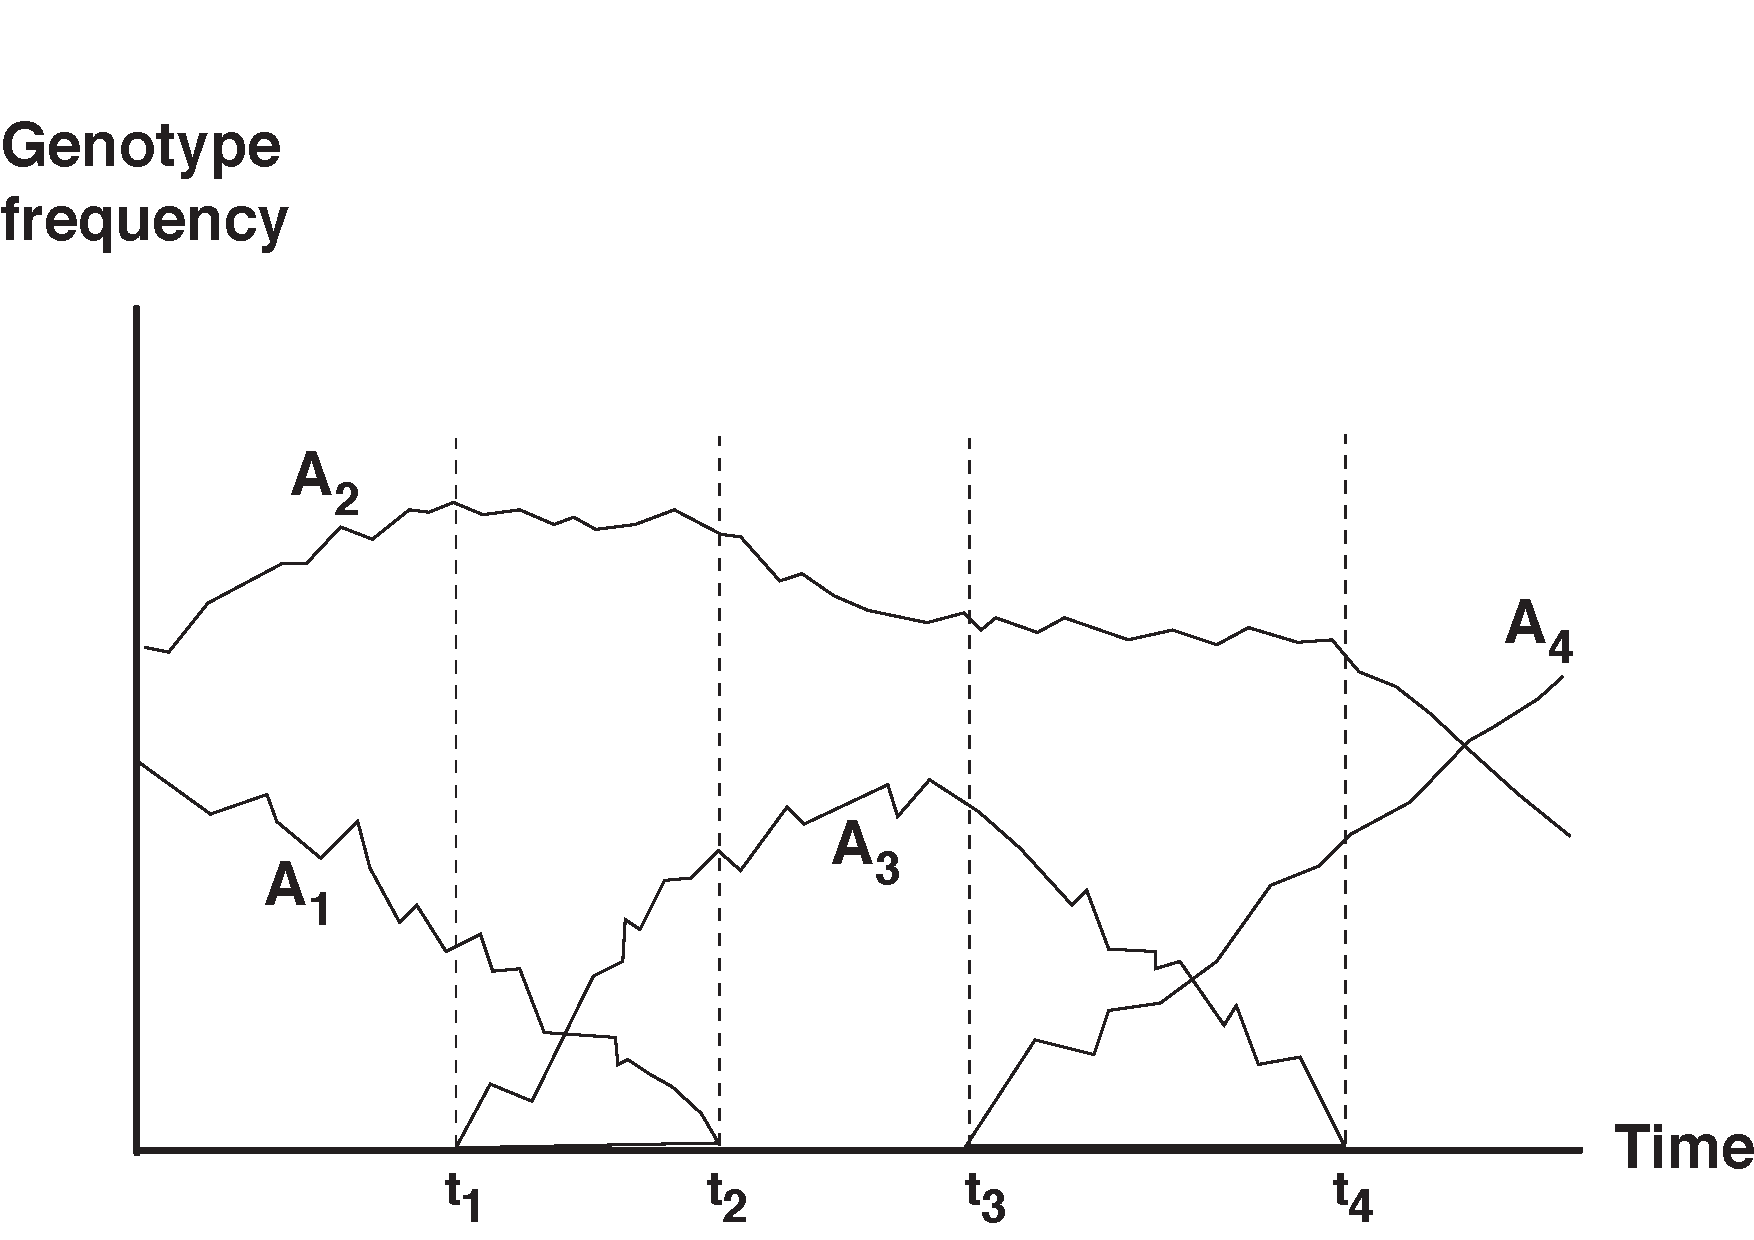
\includegraphics[bb=0 0 841 550]{figs/alleledrift.pdf}}
\caption{Genetic drift is counterbalanced by mutation resulting in the dynamic maintenance of genetic variation at a locus.}
\label{FIGdriftalleles}
\end{center}
\end{figure} 


The loss of genetic diversity caused by genetic drift  is, however, counterbalanced by the constant production of new mutations. The net result is a dynamic equilibrium where the population maintains a certain amount of variation, but the specific alleles making up this variation are changing over time. This process is illustrated in figure \ref{FIGdriftalleles} where we follow the frequencies  of alleles at a specific locus. Initially, alleles $A_1$ and $A_2$ are present. At  time $t_1$, allele $A_3$ is produced by mutation. Allele $A_1$ is lost by drift at time $t_2$, and a new allele ($A_4$) subsequently arises by mutation at time $t_3$. Later, allele $A_3$ is again lost by drift. Note that the average level of variability at the locus remains roughly constant over time, but that the actual alleles (and their frequencies) accounting for this variability changes over time.

We will now consider some aspects of how genetic drift interacts with \e{selectively neutral} mutations that are generated at a constant rate. Let us again assume that we are examining a haploid, asexual population with a constant size of $N$ individuals. Mutations are constantly being produced at a rate $\mu$. This rate is fairly constant and is perhaps mostly controlled by the interplay between the error rate of the DNA polymerase during replication and the activity of DNA repair systems. A certain fraction $f_0$ of mutations are neutral. These are produced at the rate $u=f_0\mu$.\label{PAGEuf0mu} Note that $u$ only refers to the neutral mutation rate and that this is lower than the total mutation rate. Most newly arisen  neutral mutations are immediately lost due to genetic drift, but some eventually become fixed. We are now interested in determining the over-all rate at which neutral mutations become fixed in the population. This ``rate of fixation'' tells us how quickly the DNA sequences of two isolated populations drift  apart.

The \e{number} of mutations produced per generation (at the locus we are examining) is $Nu$. For instance, if $u=2\times 10^{-7}$ mutations per generation for this locus, and if $N=10^6$ then an average of $2\times 10^{-7} \times 10^6= 0.2$ new neutral mutations will be produced at this locus per generation in the entire population (corresponding to one new neutral mutation every five generations). In the previous section we found that a single gene in a population of $N$ haploid individuals has the probability $\frac{1}{N}$ of being fixed by genetic drift. This must therefore also be the probability a newly arisen neutral mutation has of becoming fixed, since the mutant allele will initially be present as a single copy among a total of $N$ genes.  


\begin{figure}[!t]
\begin{center}
\resizebox{\textwidth}{!}{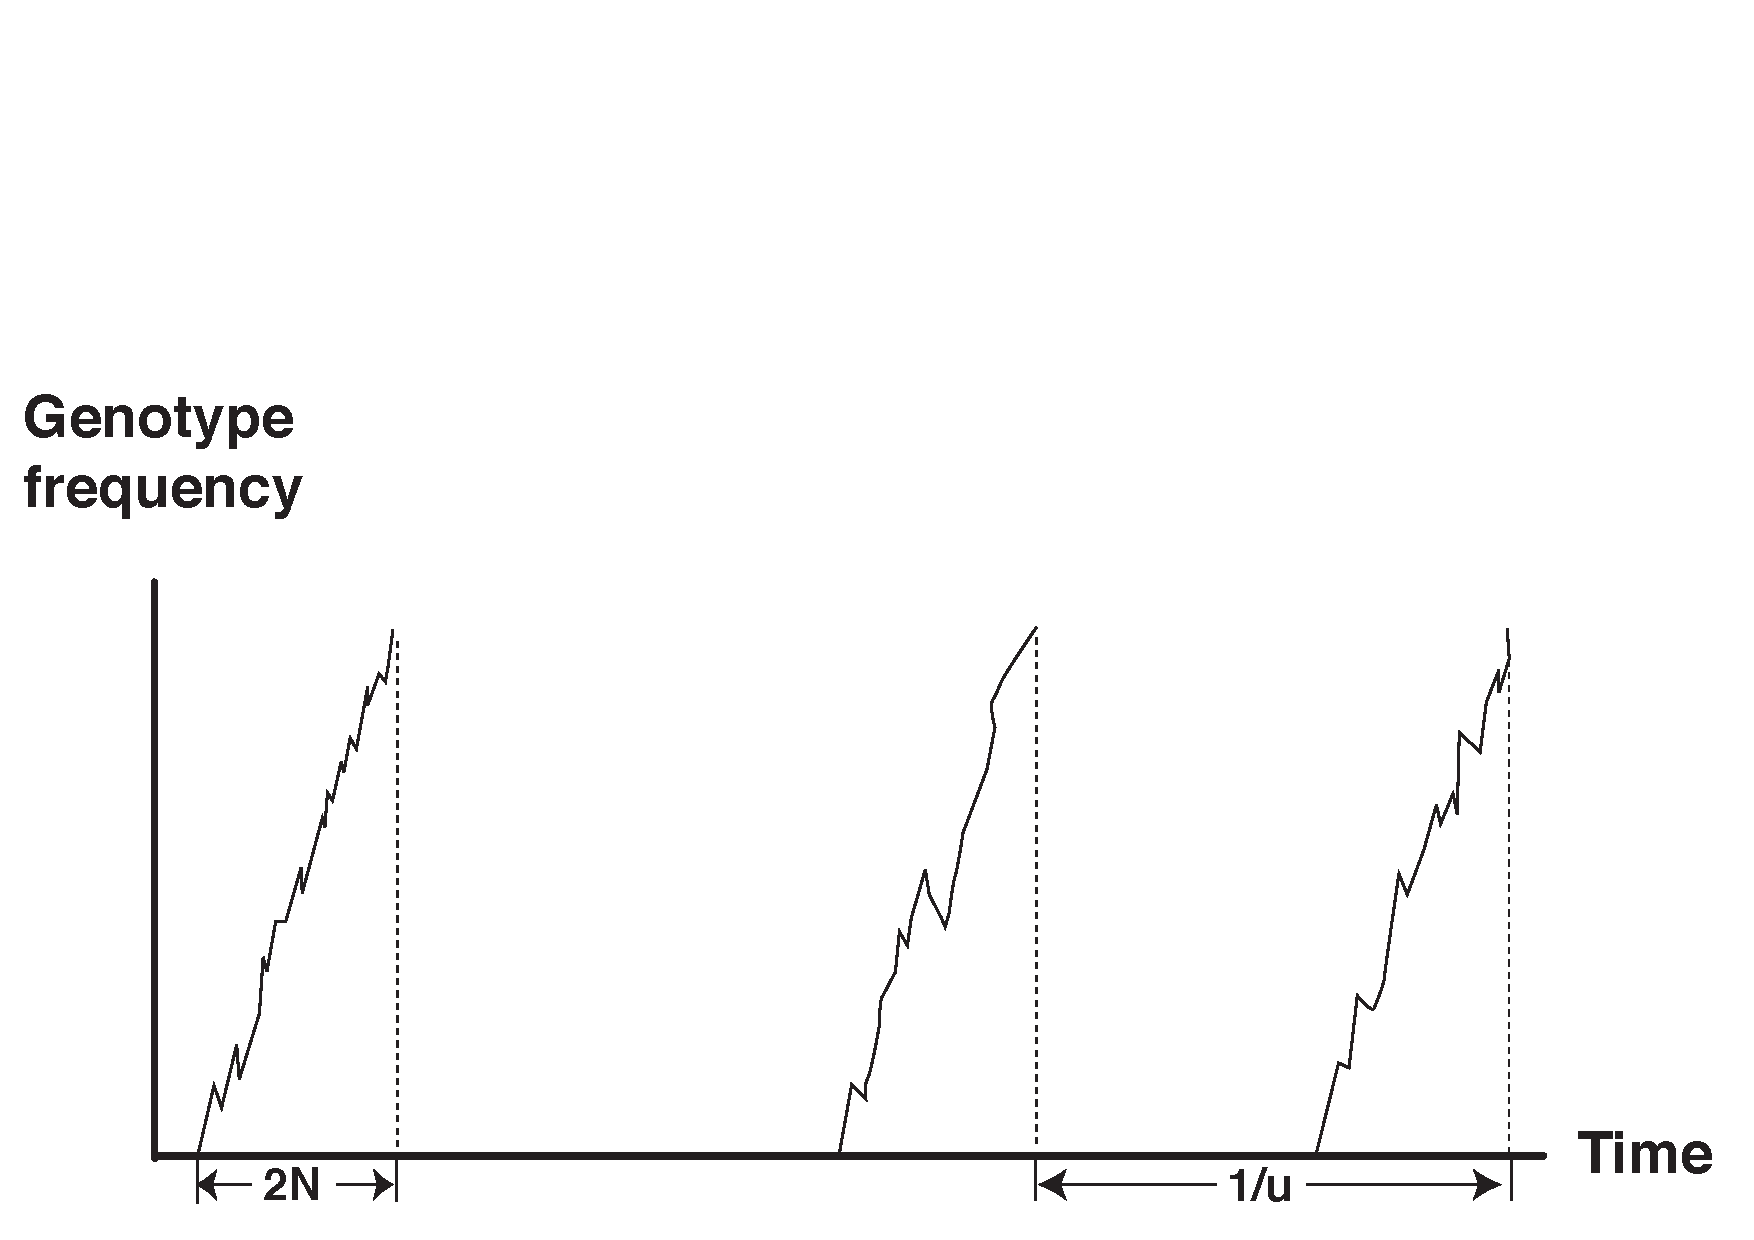
\includegraphics[bb=0 0 850 420]{figs/fixvsmut.pdf}}
\caption{The average time it takes for a neutral mutation  to reach fixation (in a population of haploid organisms) is $2N$. The average time between the fixation of different alleles at a locus is $1/u$.}
\label{FIGfixtime}
\end{center}
\end{figure} 

Recall that the rate of fixation is the number of new mutations that become fixed in a given population per generation (or any other unit of time). We can now determine this rate simply by multiplying the number of mutations produced per generation ($Nu$) by the probability that a mutation eventually becomes fixed ($\frac{1}{N}$). Denoting the rate of fixation by $k$ we therefore have:
%
\begin{equation}
k=\frac{1}{N}u N = u
\end{equation}
%
This simple but slightly surprising result shows that the rate, at which neutral mutations become fixed, is independent of the population size. Moreover, the rate of fixation is simply equal to $u$ - the neutral mutation rate. 

Note that the average time between fixation of different alleles at a locus is $t=\frac{1}{k}=\frac{1}{u}$. In our example from before, we have that $k=u={2\times 10^{-7}}$ fixed mutations per generation. The average time between fixations is therefore $t=\frac{1}{k}=\frac{1}{2\times 10^{-7}}=5,000,000$ generations per fixed mutation (at this locus). You should distinguish between the average time it takes for a mutation to reach fixation ($2N$ generations in a haploid) and the average time \e{between} fixation of different mutants ($\frac{1}{k}$; figure \ref{FIGfixtime}). 

\section{The Neutral Theory \label{SECneutheory}}\index{Neutral theory} 

Different ideas about the degree of polymorphism in real populations have been entertained at various times in the history of evolutionary theory. During the early days of the modern synthesis, it was generally believed that natural selection very quickly removed any disadvantageous alleles, and that a single predominant allele (the so-called ``wild-type'') was present at most loci. Occasionally an advantageous mutation would arise, and it would then very quickly be brought to fixation, replacing the previous wild-type in the process. This viewpoint is now referred to as the ``Classical School''.

In contrast to this view, the so-called ``Balance School'' believed that an appreciable amount of polymorphism was present in real populations. It was believed that polymorphism was being actively maintained by natural selection. One way in which selection can maintain several alleles in a population of diploid organisms is if heterozygotes are more fit than homozygotes, but there are also other selection-based scenarios with this outcome. 

According to both schools of thought, essentially all evolutionary change (meaning change in genotype frequencies) was brought about by natural selection. The phenomenon of drift was not believed to play a significant  role, since it was assumed that two alleles were very unlikely to have the same fitness. At the time it was not possible to directly measure molecular diversity. 

When the first electrophoretic studies of protein polymorphism  were published in the 1960's, the level of  genetic diversity was  much higher than anticipated by adherents of either school of thought. The classic hypothesis was obviously wrong (as there was in fact a great deal of polymorphism at many loci), but even the balance theory did not seem to be able to account for the observed levels of polymorphism. This led several authors (among them most prominently Motoo Kimura) to propose that perhaps most of the observed molecular polymorphism was in fact neutral and therefore had no effect on fitness. 

According to this so-called ``Neutral Theory'' of molecular evolution most mutations are disadvantageous and are quickly removed by natural selection, a vanishingly small proportion are advantageous and are quickly brought to fixation, while the vast majority of fixed (and therefore observed) mutations are selectively neutral. That most mutations are disadvantageous and rarely observed is in agreement with the previously prevalent views (now referred to as ``selectionist''). Selectionists and neutralists also agree that adaptation must be the result of advantageous mutations that are brought to fixation by natural selection. The main point of difference concerns the \e{fraction} of mutations that are advantageous: the extreme selectionist view is that almost all observed mutations are advantageous, while the neutralist believes that practically all observed mutations are neutral with respect to fitness. Today, we have many examples of mutations that appear to have been fixed by natural selection, but there is also a great deal of evidence for the importance of neutral mutation and genetic drift. The truth probably lies somewhere between the two extreme viewpoints.

\section{The Molecular Clock}\index{Molecular clock}\index{Clock!molecular}


\begin{figure}[!t]
\begin{center}
\resizebox{\textwidth}{!}{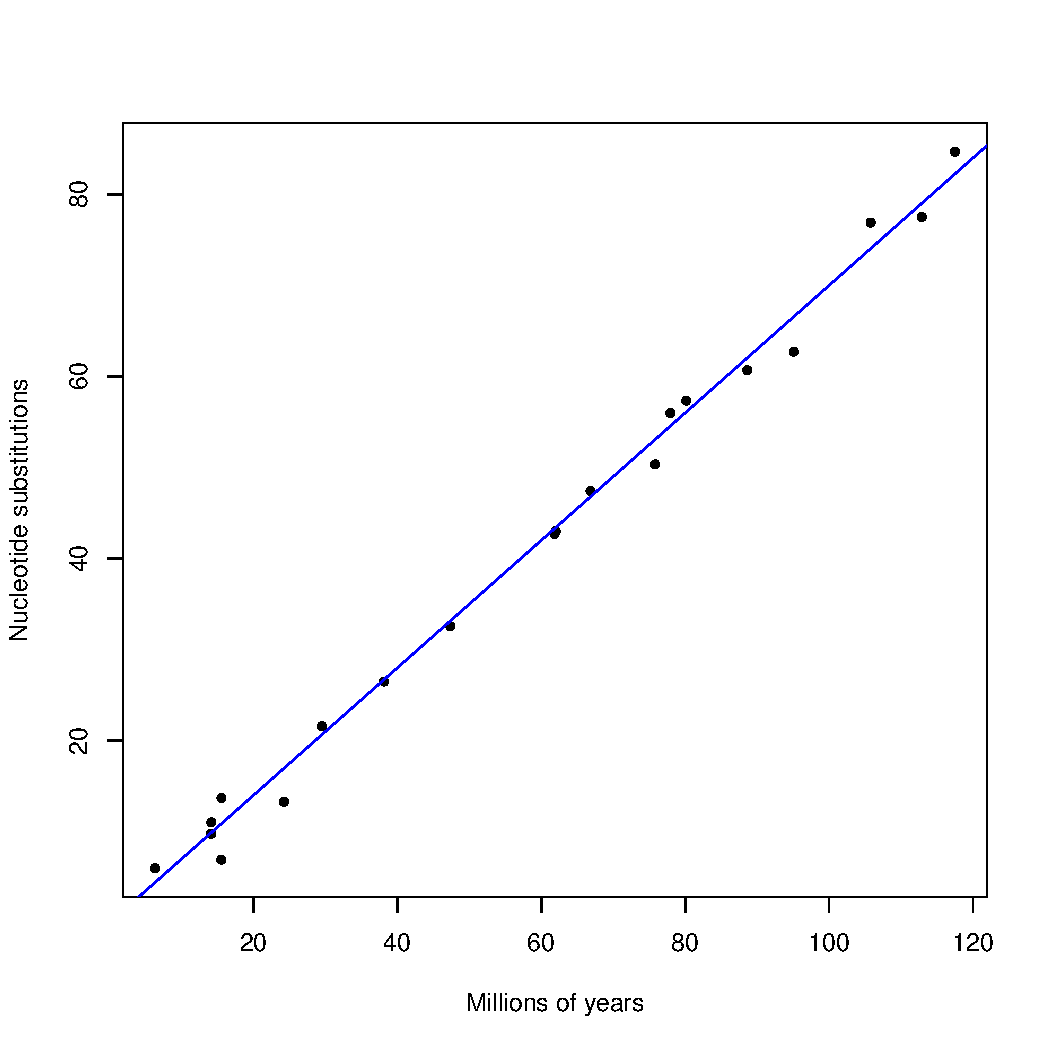
\includegraphics{figs/molecularclock.pdf}}
\caption{The molecular clock. Genetic distance (number of nucleotide replacements) increases approximately linearly with divergence time}
\label{FIGmoleclock}
\end{center}
\end{figure} 


In addition to the issue of the surprisingly high level of polymorphism, another observation was also taken as evidence for the neutral theory---the constancy of the rate of molecular evolution. 

If a particular DNA or protein sequence is examined in a number of species, then it is---for each pair of species---possible to determine (1) the approximate time since the species diverged, and (2) the number of differences between the sequences. Strikingly it was observed that if divergence time was plotted against genetic  distance for many pairs of species, then the points would fall on a straight line (Figure \ref{FIGmoleclock}).

Since genetic distance is approximately proportional to divergence time, it appears that molecular evolution must be proceeding at a roughly constant rate. If this is true of most molecular evolution, then sequences may be used to estimate approximate divergence times for species that lack an informative fossil record. 

An approximately  constant rate of molecular evolution is exactly what would be expected if most mutations are neutral: as was shown in section \ref{SECdriftmut} above neutral mutations are fixed at a constant rate $k$ regardless of population size. (Note that, obviously, neutral mutations are not produced at a perfectly constant rate---they appear at random intervals. But if they are observed over sufficiently long periods of time, then the rate of change will appear to be approximately constant. This has been described as a ``stochastic clock''). 

This rate constancy would, however,  not be expected if the selectionist scenario is correct. If most substitutions are the result of natural selection, then we would assume that the rate of evolution is heavily influenced by environmental change (where the word ``environment'' includes the impact of other living organisms). Intuitively, it  seems unlikely that the rate of environmental change is sufficiently stable to produce the constant rate of molecular evolution that has been observed in a wide range of organisms, and over long periods of time. 

There are a number of things that should be noted with regard to the molecular clock. First, molecular clocks do not run at the same speed in different sequences. Generally, it appears that less constrained sequences evolve faster. Secondly, things are not quite as tidy as figure \ref{FIGmoleclock} implies. There are many examples where evolution does not proceed at a constant rate. However, it is probably fair to say that all in all, the examples that we \e{do} have of rate constancy are sufficiently striking to require some sort of explanation. Finally, selectionist explanations for the molecular clock have also been proposed, although generally these seem to be slightly \e{ad hoc} and unsatisfactory.




%\section{Sexual Reproduction: The Hardy-Weinberg Principle}

%We will now consider the situation for diploid organisms with sexual reproduction. Let us again assume that there are two different alleles in the population---A and a. Different individuals will have one of the following three (diploid) genotypes: AA, aa, or Aa. Let us say that we start our examination immediately prior to gamete formation. At this time the three genotypes are present in the population in the proportions $P_{AA}$, $P_{aa}$, and $P_{Aa}$, (where $P_{AA}+P_{aa}+P_{Aa}=1$). As usual, we denote the initial size of the entire population $N_0$. 

%Let us start out with computing the initial \emph{allele} frequencies ($p$ and $q$) from the \emph{genotype} frequencies mentioned above. First, note that since there are $N_0$ diploid organisms, then there will be a total of $2 N_0$ gene copies in the population. In each of the $N_0 P_{AA}$ individuals with genotype AA there will be two copies of the A allele. This corresponds to $2N_0 P_{AA}$ copies of the A allele. Similarly, each of the $N_0 P_{Aa}$ individuals with genotype Aa will harbor one copy of the A allele, corresponding to $N_0 P_{Aa}$ copies of the A allele. There are of course no A alleles in the aa individuals. We therefore have that the initial number of A alleles in the population is:
%%
%\begin{displaymath}
%N_A = 2N_0 P_{AA}  + N_0 P_{Aa} 
%\end{displaymath}
%%
%Since the total number of gene copies (A and a) is $2 N_0$, the initial frequency of the A allele can be computed as:
%%
%\begin{equation*}
%p = \frac{2 N_0 P_{AA} +  N_0 P_{Aa}}{2 N_0}
%\end{equation*}
%This can be simplified by eliminating $2N_0$:
%\begin{equation}
%\label{EQhardypA}
%p = P_{AA} + \tfrac{1}{2} P_{Aa}
%\end{equation}
%%
%Similarly the initial frequency of a must be:
%%
%\begin{equation}
%\label{EQhardypa }
%q = P_{aa} + \tfrac{1}{2} P_{Aa}
%\end{equation}
%%
%These equations means that we can deduce the allele frequencies from the genotype frequencies. The opposite is not always the case. For instance, all A alleles could be present in homozygotes, but they could also all be present in heterozygotes. Note that the frequencies of the two alleles sum to one:
%%
%\begin{align*}
%p + q &= \left(P_{AA} + \tfrac{1}{2} P_{Aa}\right) + \left(\tfrac{1}{2} P_{Aa} + P_{aa}\right)\\
%		&= P_{AA} + P_{Aa} + P_{aa}\\
%		&= 1
%\end{align*}

%Let us now proceed to consider what happens to the genotype frequencies after one round of gamete formation and fertilization. We will assume that the two sexes have identical genotype frequencies (and therefore also allele frequencies) and that mating is random (an individual is equally likely to mate with any other individual regardless of genotype). Importantly, we will furthermore disregard the reproductive rate in our computations: as the analysis above has shown us, the proportions of different alleles will not change as a result of exponential growth in itself, as long as the different genotypes have the same rate of increase. We can therefore focus on the proportions and ignore the total numbers of alleles involved. 

%Regardless of the absolute number of eggs and sperm that are produced by each individual, we know that the proportion of gametes with alleles A and a will be $p$ and $q$ respectively when taken across the entire population. If we imagine that the next generation of zygotes were formed by random fusion of pairs of gametes from this pool, then it is easy to compute the genotype frequencies after mating:

%





%%%%%%%%%%%%%%%%%%%%%%%%%%%%%%%%%%%%%%%%%%%%%
%							CHAPTER
%%%%%%%%%%%%%%%%%%%%%%%%%%%%%%%%%%%%%%%%%%%%%


%	\chapter{Answers to exercises}
%		\fancyhead[LO]{Chapter X: Answers to exercises}		
%		\fancyhead[RE]{Molecular Evolution, lecture notes}
%		\input{lecturenotebookans} NOTE: file extension .ans not recognized. 
%		Rename!


%\printindex

\end{document}
 